\chapter{関連研究}
本研究では犬の一人称視点動画からの犬の活動分類を行う.人間のライフログとしての一人称動画の分類や,車載映像からの車の行動推定,第三者視点での動画分類,音声を用いた動画分類などについて紹介し,本研究との関連を述べる.

\section{タフ・ロボティクス・チャレンジ}
政府による総合科学技術・イノベーション会議が研究開発を促進している,革新的研究開発推進プログラムImPACTというプログラムがある~\cite{impact}.
「ImPACTは研究開発を促進し,持続可能な発展性のあるイノベーションシステムの実現を目指したプログラム」であり,複数の研究開発プログラムを包括している.
タフ・ロボティクス・チャレンジはそのプラグラムのうちの一つであり,遠隔自律ロボット,屋外ロボットサービス事業の実現を目指したプログラムである.
このプログラムでは首都圏直下型地震などを想定し,刻々と変化する厳しい環境下でも実用性を保つ災害救助を目的としたロボットの研究開発が行われている.倒壊家屋や配管内を探索するロボット,悪天候でも飛行するドローンなどを用いての計測や認識,マッピング,活動支援などが達成目標として掲げられる.

\subsection{サイバー救助犬}
サイバー救助犬の研究はタフ・ロボティクス・チャレンジの一つである.災害救助用サイボーグ犬の開発を見据え,その足がかりとして研究されている.
サイバー救助犬の技術的達成目標は``救助犬の行動と状態の計測・伝送・認識・マッピング(運動・映像・声・生体信号)と制御による、救助活動支援''とされており,レスキュー犬の行動をモニタリングするために,濱田,大野らによって装着型計測・記録装置が開発された~\cite{dog01}.
図\ref{cyberdog}にレスキュー犬に装着可能な軽量な行動計測スーツを示す.これを着用したレスキュー犬はサイバー救助犬とも呼ばれる.
サイバー救助犬は各種センサを用いた計測データを記録し,リアルタイムに映像などのデータの無線配信が可能である.そのため,人の目の及ばない範囲でレスキュー犬が活動する際にもレスキュー犬の行動やその周辺環境などが把握可能である.

\begin{figure}[htbp]
 \begin{center}
  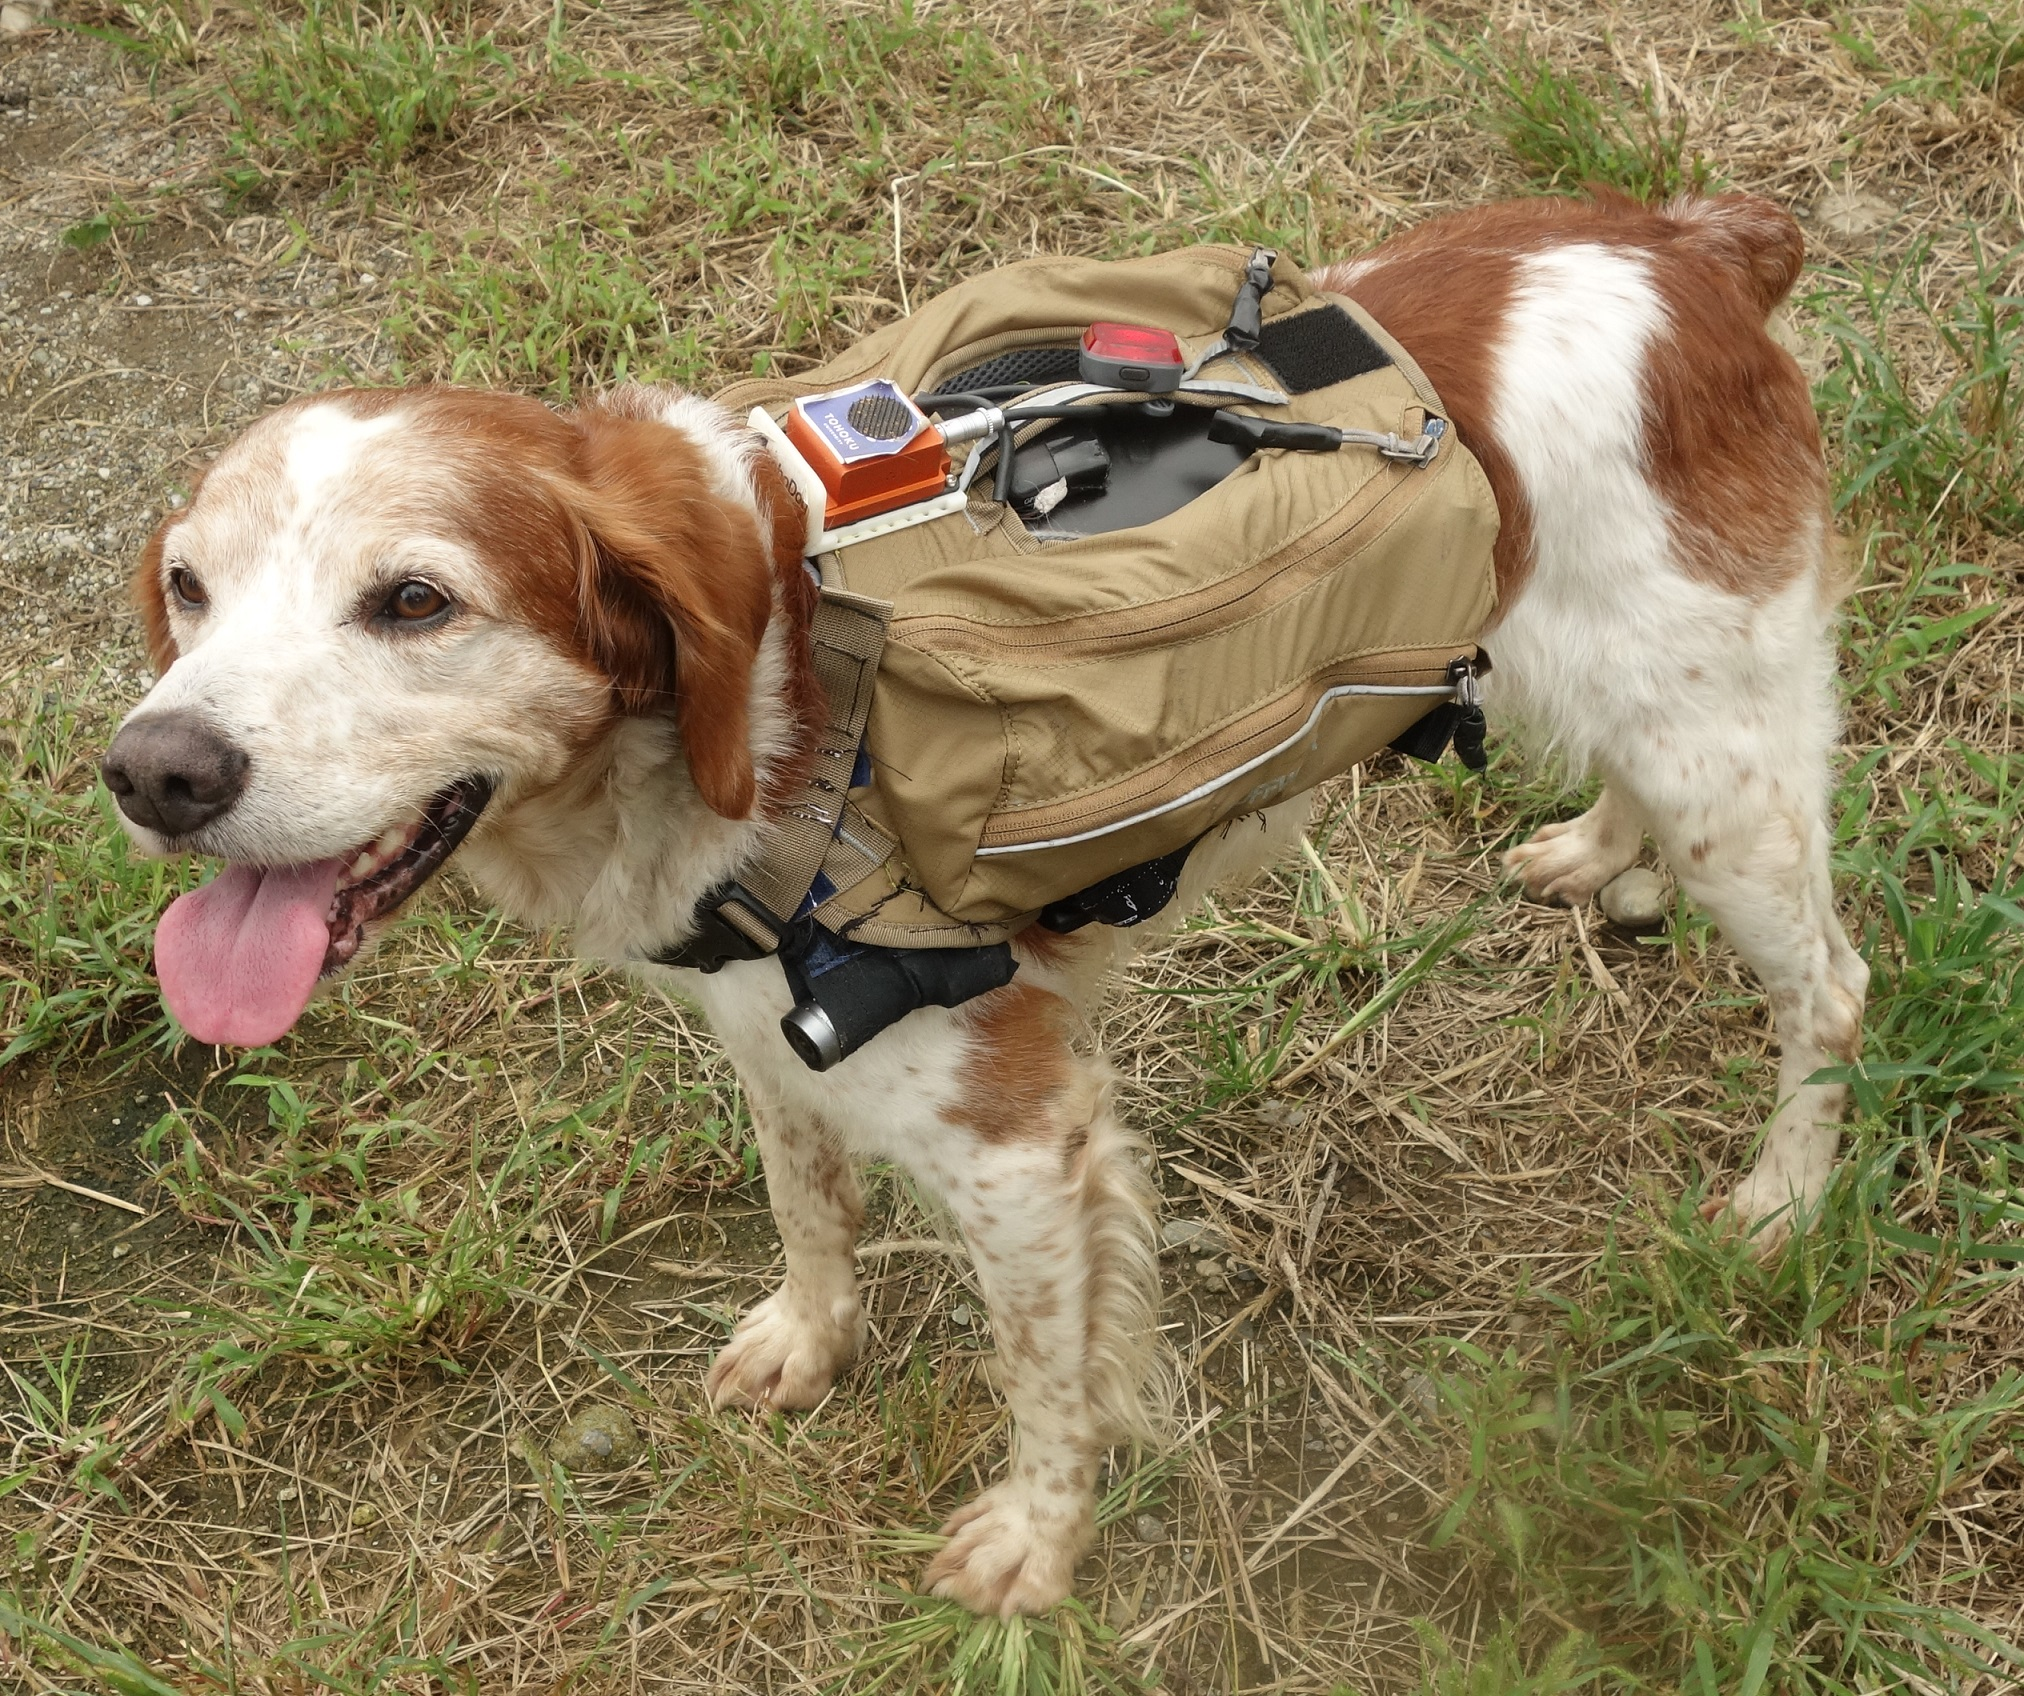
\includegraphics[width=9cm]{./Figures/cyberdog.eps}
  \caption{装着型計測・記録装置~\cite{dog01}より引用}
  \label{cyberdog}
 \end{center}
\end{figure}

\section{動画認識}
犬一人称視点映像の動きや音声の特徴は,レスキュー犬の周辺環境を知るための重要な手掛かりの1つである.
レスキュー犬の一人称動画に限らず,動画から特徴を取得してその内容を分類する類の研究は行われている.
\subsection{動作認識}
映像から動き特徴を抽出する手法は大きく分けて2つある.
1つはあらかじめ動画を複数枚の画像に分割してから特徴量を抽出する手法である.
もう1つは動画から直接特徴量を抽出する手法である.
前者は既存の画像認識の技術を簡単に流用でき,入力データが比較的小さいので学習コストが低い.
対して後者はフレーム間の情報を考慮できるが,動画を直接入力データとするため学習コストが非常に高い.
%\subsubsection{Two-stream convolutional network}
\subsubsection{動画内の連続した静止画間の動き推定}
動画の動き特徴を取得して表現する方法として\cite{Zach2007optical}がある.
これは静止画像の特徴点と連続した次の静止画像の特徴点から移動ベクトルを求め,ピクセル毎にその分布を取得する.
移動ベクトルの曖昧な部分も周辺のベクトル分布を加味し平滑化することでより滑らかな分布を取得している.
本研究では,動画からoptical flow画像を生成する際にこの手法を用いる.
\subsubsection{静止画を入力とする動画認識}
事前に動画から静止画を切り出してから特徴を抽出し学習する手法としては~\cite{simonyan2014two}, \cite{wang2015towards}が挙げられる.
Simonyanらによるtwo-stream CNN~\cite{simonyan2014two}は,1つの動画から通常のRGB画像とoptical flow画像を抽出し,
それぞれを入力とする個々のネットワークを学習することで動き情報を考慮して動画を分類する手法である.
図~\ref{2st_network}に\cite{simonyan2014two}のネットワーク構造を示す.
この手法では,入力となる動画から静止画を切り出し,さらにoptical flow画像を生成している.
これらをそれぞれのストリームの入力とし,動画のクラスを出力とする.入力画像に対し複数回畳み込み,全結合層に通した後Softmax関数でクラス毎の確率を計算することでクラスの判定を行う.

Two-streamをベースにした派生ネットワークの研究は多く、Convolutional Two-Stream Network Fusion~\cite{a}もその1つである。
これは,それぞれのストリームの畳み込み層の出力を結合し,その後FC層を追加することでUCF-101と呼ばれる動画分類の標準ベンチマークデータセットの分類において最高精度を達成した.

本研究でもこのTwo-stream CNNをベースにしたアーキテクチャを構築し,クラス推定へアプローチする.
\begin{figure}[htbp]
 \begin{center}
  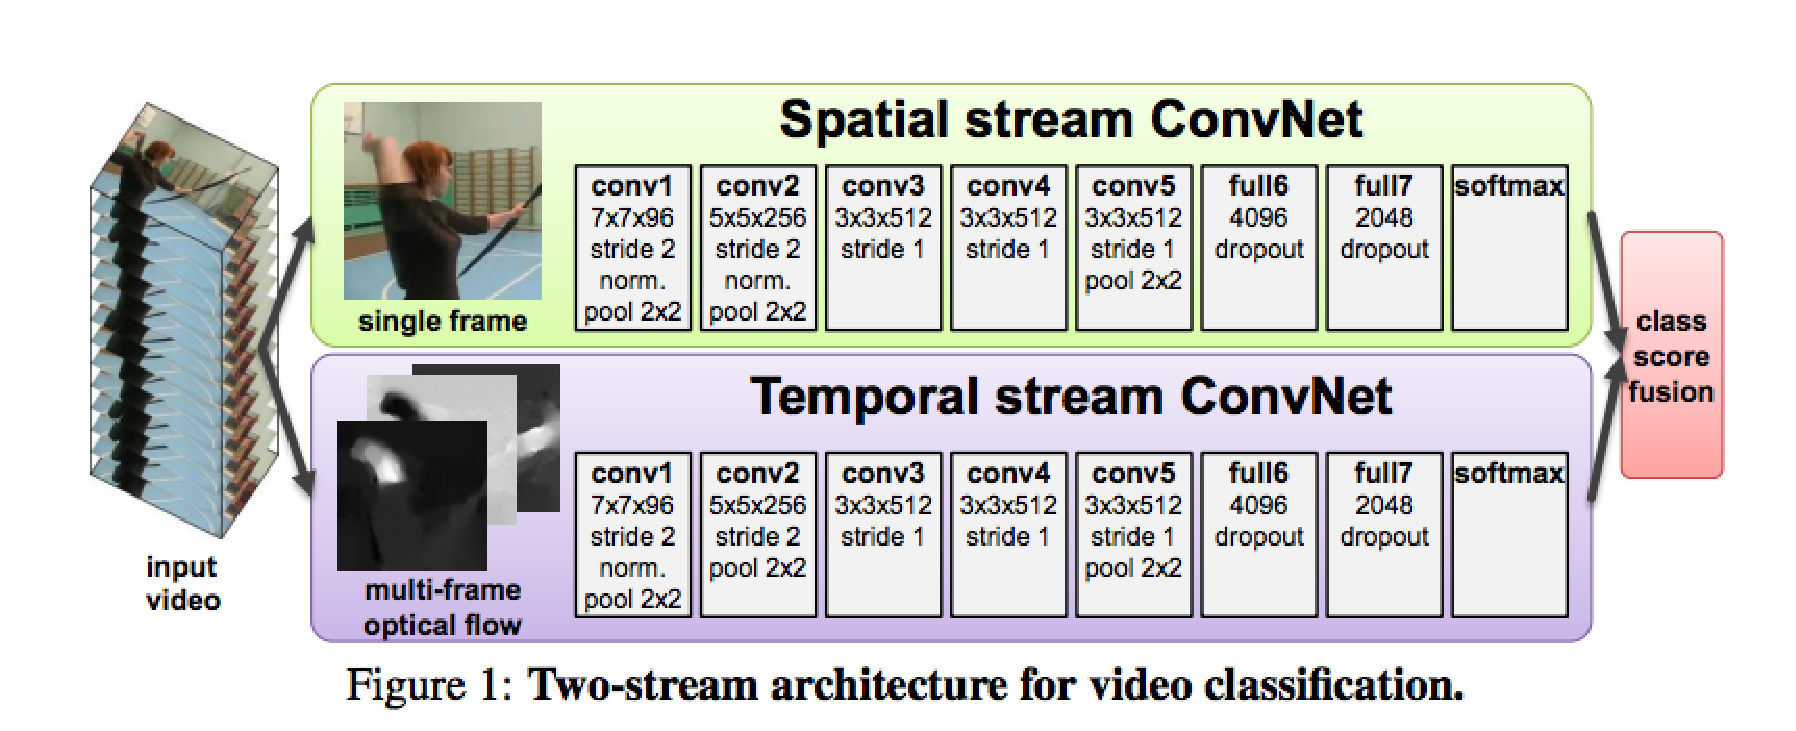
\includegraphics[width=12cm]{./Figures/two-stream.eps}
  \caption{Two-stream CNNの アーキテクチャ~(\cite{simonyan2014two}より引用).切り出したRGB画像とoptical flow画像を個々のネットワークに入力し、出力を合わせている.}
  \label{2st_network}
 \end{center}
\end{figure}

\subsubsection{動画を入力とする動画認識}
動画から直接特徴を抽出して学習する手法としてはTranらによる3D Convolution がある~\cite{tran14}.
画像に対して2次元であったフィルターを3次元形状に拡張することで,縦横の空間以外である時間方向への広がりを持って特徴抽出が可能になった.
図~\ref{3dconv_image}に3D Convolutionalの詳細を示す.

Two-stream convolution networkのストリームへの入力が画像であったのに対し,この手法では動画を直接の入力とする.
本研究では画像を入力とする点で,この手法とは異なっている.

\begin{figure}[htbp]
 \begin{center}
  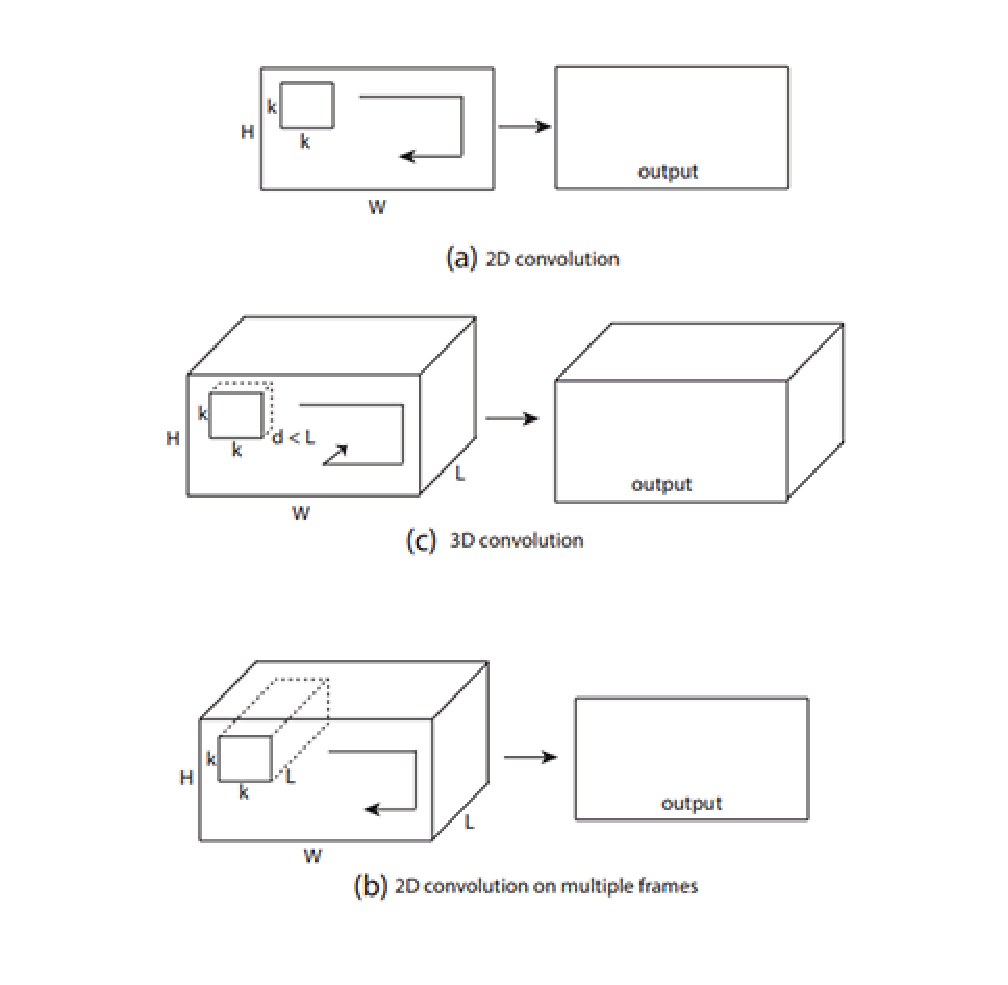
\includegraphics[width=12cm]{./Figures/3dconv.eps}
  \caption{3D Convolutionの詳細~(\cite{tran14}より引用).2D Convolutionでは縦横方向の畳み込みを行っており,3D Convolutionでは加えて時間方向への畳み込みを行っている.}
  \label{3dconv_image}
 \end{center}
\end{figure}


\subsubsection{一人称映像からの行動分類}
動作認識の中でも,一人称視点の映像からFarst Personがどのような行動を行なっているのか分類する研究がある~\cite{minghuang2016fpar}\cite{gedas2017dblp}.
Minghuangら\cite{minghuang2016fpar}は,最近の研究から一人称映像行動の分類において,手の位置・手の動き・対象の物体・カメラの動きが動作認識に重要であるとしてこれらを統合したtwin stream networkを提案した.
twin stream networkのアーキテクチャを図~\ref{twinst_image}に示す.
腕領域と物体をCNNを通し推定した後,さらにCNNを通しoptical flow画像のCNN出力結果と統合している.最終的な出力は物体認識結果と動作認識結果,それらを合わせた行動推定結果の3つである.
本研究では対象となる物体もなく,カメラと犬の位置関係が決まっているため腕領域のように犬領域の推定はしない.
\begin{figure}[htbp]
 \begin{center}
  \includegraphics[width=12cm]{./Figures/goingtodeeper.eps}
  \caption{twin stream networkの詳細~(\cite{minghuang2016fpar}より引用).腕領域のセグメンテーションネットワーク,関連物体の位置推定ネットワーク,物体推定ネットワーク,動作ネットワークが組み合わせられている.同時に物体推定と行動推定を行うことで動作認識を行なっている.}
  \label{twinst_image}
 \end{center}
\end{figure}

\subsubsection{犬一人称視点からの行動予測}
犬一人称映像からの犬の行動予測を行なった研究に\cite{whoretthedog}がある.
%Modeling Dog Behavior From Visual Data
これは,犬の行動をモデリングし,犬が次にどのような道をたどり行動するかを予測している.

しかし,これらの研究は犬の行動のモデリングであり,犬の周辺環境の推定などは行っていない.
また,入力は動画像のみであり,音声などのデータも利用していない.
レスキュー犬の課題には犬の周辺環境情報や映像からだけでは判断できない情報の取得が含まれている.
例えばレスキュー犬は要救助者を発見するとその場で待機し吠え続けるように訓練されている.
このように,映像データからだけではなく,音声データ,および慣性データ・GPSデータなどの情報を複合的に用いてレスキュー犬の状態を判断しなければならない.
本研究は映像と音声からなるマルチモーダルな情報を入力とした犬の行動推定を目的としている. 


\subsection{音声分類}
音声と画像から特徴を抽出する研究には以下のようなものがある.
\subsubsection{Sound Net}
音声をクラス分類する研究としてAyterらによるSound Netがある~\cite{aytar2016soundnet}.
動画から音声と画像を取り出し,画像を教師データとし,音声は生徒データとして出力が等しくなるように学習している.
この手法は音響シーン分類,物体分類の標準ベンチマークにおいて教師あり学習の最高精度を達成した.
図~\ref{soundnet_network}にSound Netのネットワーク構造を示す.
本研究では音声のみからの行動推定は目的としない.しかし,音声の意味的情報は動画認識に重要であることが明らかにされている.
音声を入力とするストリームの構築にあたり,Sound Netで用いられている音声畳み込みネットワークを参考にした.
\begin{figure}[htbp]
 \begin{center}
  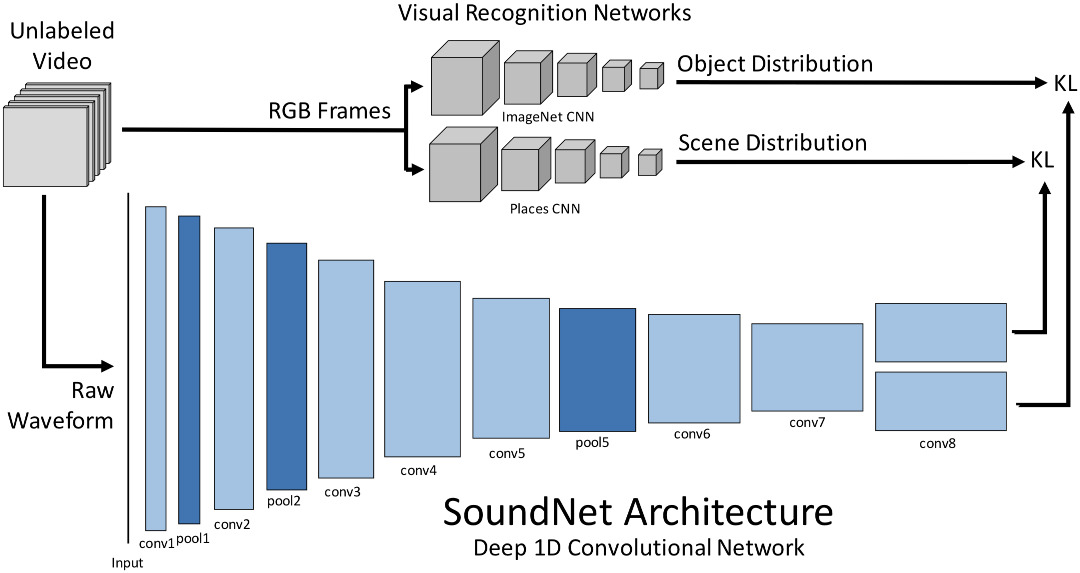
\includegraphics[width=15cm]{./Figures/soundnet.eps}
  \caption{Sound Netのアーキテクチャ~(\cite{aytar2016soundnet}より引用).動画から映像と音声を切り分け,音声に対して1次元の畳み込みを行なっている.}
  \label{soundnet_network}
 \end{center}
\end{figure}

\subsubsection{Audio-Visual Scene Analysis}
音声と動画を紐づけて,その関係を明らかにする研究としてOwensらによるAudio-Visual Scene Analysisがある~\cite{multisensory2018}.
映像内の音源特定,音声からの動作認識,複数の話者が個々の画面にいる際の話者の特定を行なっており,音声と映像の関連性を示している.
具体的な図を~\ref{audio_visual}に示す.
\begin{figure}[htbp]
 \begin{center}
  \includegraphics[width=15cm]{./Figures/audio_visual.eps}
  \caption{Audio-Visual Scene Analysis~(\cite{multisensory2018}より引用).}
  \label{audio_visual}
 \end{center}
\end{figure}
